\section{HTTP and the Web}
\subsection{Precursors}
\begin{itemize}[nosep]
    \item 1945, Vannevar Bush, Memex:
          \begin{itemize}[nosep]
              \item ``\textit{a device in which an individual stores all his books, records, and communications, and which is mechanized so that it may be consulted with exceeding speed and flexibility}''
          \end{itemize}
    \item Precursors to hypertext
          \begin{itemize}[nosep]
              \item ``\textit{The human mind [\dots] operates by association. WIth one item in its grasp, it snaps instantly to the next that is suggested by the association of thoughts, in accordance with some intricate web of trails carried by the cells of the brain}''
          \end{itemize}
    \item Read his 1945 essay, ``As we may think''
          \begin{itemize}[nosep]
              \item \url{https://www.theatlantic.com/magazine/archive/1945/07/as-we-may-think/303881/}
          \end{itemize}
\end{itemize}
\subsection{Tim Berners-Lee}
\begin{itemize}[nosep]
    \item Physicist at CERN, trying to solve real problem
          \begin{itemize}[nosep]
              \item Distributed access to data
          \end{itemize}
    \item WWW: distributed database of pages linked thruogh the Hypertext Transfer Protocol
          \begin{itemize}[nosep]
              \item First HTTP implementation: 1990
              \item HTTP/0.9 -- 1991
                    \begin{itemize}[nosep]
                        \item Simple \mintinline{http}|GET| command
                    \end{itemize}
              \item HTTP/1.0 -- 1992
                    \begin{itemize}[nosep]
                        \item Client/server information, simple caching
                    \end{itemize}
              \item HTTP/1.1 -- 1996
                    \begin{itemize}[nosep]
                        \item Extensive caching support
                        \item Host identification
                        \item Pipelined, persistent connections, \dots
                    \end{itemize}
          \end{itemize}
\end{itemize}
\subsection{Components}
\begin{itemize}[nosep]
    \item Content
          \begin{itemize}[nosep]
              \item Objects (may be static or dynamically generated)
          \end{itemize}
    \item Clients
          \begin{itemize}[nosep]
              \item Send requests / receive responses
          \end{itemize}
    \item Servers
          \begin{itemize}[nosep]
              \item Receive requests / send responses
              \item Store or generate content
          \end{itemize}
    \item Proxies
          \begin{itemize}[nosep]
              \item Placed between clients and servers
              \item Provide extra functions
                    \begin{itemize}[nosep]
                        \item Caching, anonymization, logging, transcoding, filtering access
                    \end{itemize}
              \item Explicit or transparent
          \end{itemize}
\end{itemize}
\subsection{Ingredients}
\begin{itemize}[nosep]
    \item HTTP
          \begin{itemize}[nosep]
              \item Hypertext Transfer Protocol
          \end{itemize}
    \item HTML
          \begin{itemize}[nosep]
              \item Language for description of content
          \end{itemize}
    \item Names (mostly URLs)
\end{itemize}
\subsection{URLs}
\textcolor{blue}{\texttt{protocol://[name@]hostname[:port]/directory/resource?k1=v1\&k2=v2\#tag}}
\begin{itemize}[nosep]
    \item \emph{Name} is for possible client identification
    \item \emph{Hostname} could be an IP address
    \item \emph{Port} defaults to protocol default (e.g. 80)
    \item \emph{Directory} is a path to the resource
    \item \emph{Resource} is the name of the object
    \item \emph{?parameters} are passed to the server for execution
    \item \emph{\#tag} allows jumps to named tags within document
\end{itemize}
\subsection{Examples of URLs}
\begin{itemize}[nosep]
    \item \url{http://www2.cs.uh.edu/~gnawali/courses/cosc4377-s12/schedule.html}
    \item \url{http://en.wikipedia.org/wiki/Domain_name#Top-level_domains}
    \item \url{http://www.uh.edu/search/?q=computer+science&x=0&y=0}
\end{itemize}
\subsection{HTTP}
\begin{itemize}[nosep]
    \item Important properties
          \begin{itemize}[nosep]
              \item Client-server protocol
              \item Protocol (but not data) in ASCII
              \item Stateles
              \item Extensible (header fields)
          \end{itemize}
    \item Server typically listens on port 80
    \item Server sends response, may close connection (client may ask it to stay open)
    \item Version 1.1 in use by less than 45\% of websites, version 2 in use by over 45\% of websites, version 3 in use by 5.8\% of websites
\end{itemize}
\subsection{Steps in HTTP Request}
\begin{itemize}[nosep]
    \item Open TCP connection to server
    \item Send request
    \item Receive response
    \item TCP connection terminates
          \begin{itemize}[nosep]
              \item How many RTTs for a single request?
          \end{itemize}
    \item You may also need to do a DNS lookup first!
\end{itemize}
\begin{figure}[H]
    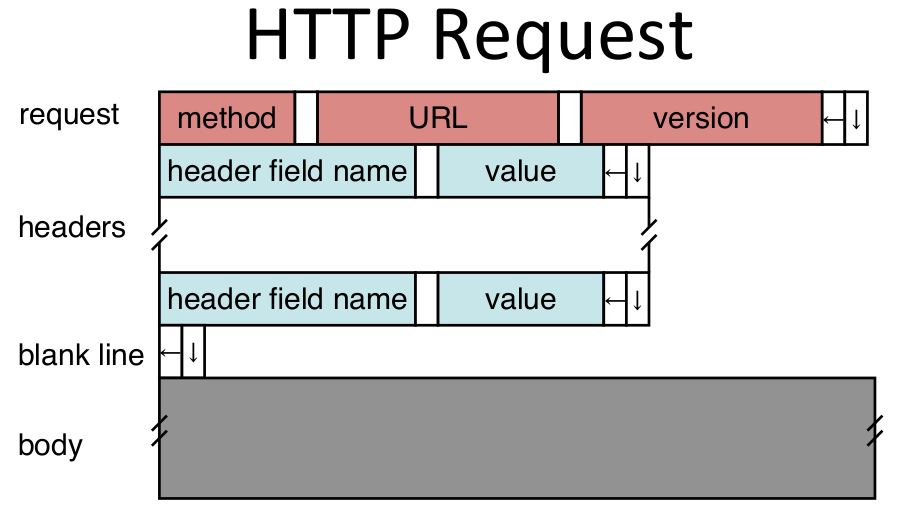
\includegraphics[width=\textwidth]{lazy/httprequest.png}
\end{figure}
\begin{itemize}[nosep]
    \item Method:
          \begin{itemize}[nosep]
              \item \mintinline{http}|GET|: current value of resource, run program
              \item \mintinline{http}|HEAD|: return metadata assocated with a resource
              \item \mintinline{http}|POST|: update a resource, provide input for a program
          \end{itemize}
    \item Headers: useful info for proxies or the server
          \begin{itemize}[nosep]
              \item e.g. desired language
          \end{itemize}
\end{itemize}
\subsection{Sample Browser Request}
\begin{minted}{http}
    GET / HTTP/1.1
    Host: localhost:8000
    User-Agent: Mozilla/5.0 (Macinto ...
    Accept: text/xml,application/xm ...
    Accept-Language: en-us,en;q=0.5
    Accept-Encoding: gzip,deflate
    Accept-Charset: ISO-8859-1,utf-8;q=0.7,*;q=0.7
    (empty line)
\end{minted}

\subsection{Sample HTTP Response}
\begin{minted}{http}
    HTTP/1.0 200 OK
    Date: Wed, 25 Jan 2012 08:11:09 GMT
    Expires: -1
    Cache-Control: private, max-age=0
    Content-Type: text/html; charset=ISO-8859-1
    Set-Cookie: PREF=ID….
    P3P: CP="This is not a P3P policy! See http://
    www.google.com/support/accounts/bin/answer.py?
    hl=en&answer=151657 for more info."
    Server: gws
    X-XSS-Protection: 1; mode=block
    X-Frame-Options: SAMEORIGIN
    <!doctype html><html><head><meta http-equiv="content-type"
    content="text/html; charset=ISO-8859-1"><meta…>
\end{minted}
\begin{figure}[H]
    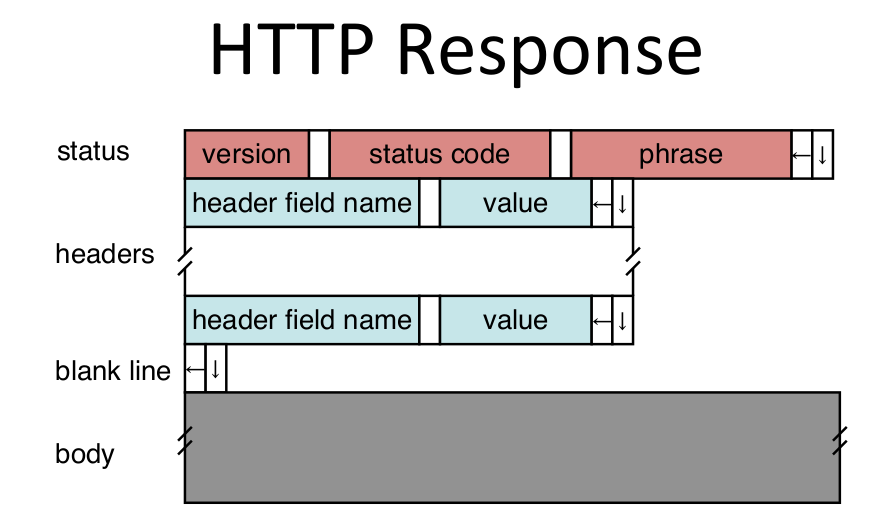
\includegraphics[width=\textwidth]{lazy/httpresponse.png}
\end{figure}
\begin{itemize}[nosep]
    \item Status Codes:
          \begin{itemize}[nosep]
              \item 1xx: Information, e.g. 100 Continue
              \item 2xx: Success, e.g. 200 OK
              \item 3xx: Redirection, e.g. 302 Found (elsewhere)
              \item 4xx: Client Error, e.g. 404 Not Found
              \item 5xx: Server Error, e.g. 503 Service Unavailable
          \end{itemize}
\end{itemize}
\subsection{HTTP is Stateless}
\begin{itemize}[nosep]
    \item Each request/response treated independently
    \item Servers not required to maintain state
    \item This is good!
          \begin{itemize}[nosep]
              \item Improves server scalability
          \end{itemize}
    \item This is also bad\dots
          \begin{itemize}[nosep]
              \item Some applications need persistent state
              \item Need to uniquely identify user to customize content
              \item e.g. shopping cart, web-mail, usage tracking, (most sites today!)
          \end{itemize}
\end{itemize}
\subsection{HTTP Cookies}
\begin{itemize}[nosep]
    \item Client-side state maintenance
          \begin{itemize}[nosep]
              \item Client stores small state on behalf of server
              \item Sends request in future requests to the server
              \item Cookie value is meaningful to the server (e.g. session ID)
          \end{itemize}
    \item Can provide authentication
    \item \url{https://en.wikipedia.org/wiki/HTTP_cookie}
\end{itemize}
Where to find official HTTP specificaton?

\url{www.w3.org}
\subsection{Anatomy of a Web Page}
\begin{itemize}[nosep]
    \item HTML content
    \item A number of additional resources
          \begin{itemize}[nosep]
              \item Images
              \item Scripts
              \item Frames
          \end{itemize}
    \item Browser makes one HTTP request for each object
          \begin{itemize}[nosep]
              \item Course web page: 4 objects
              \item My facebook page this morning: 100 objects
          \end{itemize}
\end{itemize}
\subsection{AJAX}
\begin{itemize}[nosep]
    \item \emph{Asynchronous JavaScript and HTML}
    \item Based on XMLHttpRequest object in browsers, which allow code in the page to:
          \begin{itemize}[nosep]
              \item Issue a new, non-blocking request to the server, without leaving the current page
              \item Receive the content
              \item Process the content
          \end{itemize}
    \item Used to add interactivity to web pages
          \begin{itemize}[nosep]
              \item XML not always used, HTML fragments, JSON, and plain text also popular
          \end{itemize}
\end{itemize}
\subsection{HTTP Performance}
\begin{itemize}[nosep]
    \item What matters for performance?
    \item Depends on type of request
          \begin{itemize}[nosep]
              \item Lots of small requests (objects in a page)
              \item Some big requests (large download or video)
          \end{itemize}
\end{itemize}

\subsection{Small Requests}
\begin{itemize}[nosep]
    \item Latency matters
    \item RTT dominates
    \item Two major causes:
          \begin{itemize}[nosep]
              \item Opening a TCP connection
              \item Actually sending the request and receiving response
              \item And a third one: DNS lookup!
          \end{itemize}
    \item Mitigate the first one with persistent connections (HTTP/1.1)
          \begin{itemize}[nosep]
              \item Which also means you don't have to ``open'' the connection each time
          \end{itemize}
\end{itemize}

\paragraph{Browser Request}
\begin{minted}{http}
    GET / HTTP/1.1
    Host: localhost:8000
    User-Agent: Mozilla/5.0 (Macinto ...
    Accept: text/xml,application/xm ...
    Accept-Language: en-us,en;q=0.5
    Accept-Encoding: gzip,deflate
    Accept-Charset: ISO-8859-1,utf-8;q=0.7,*;q=0.7
    Keep-Alive: 300
    Connection: keep-alive
\end{minted}

\begin{itemize}[nosep]
    \item Second problem is that requests are serialized
          \begin{itemize}[nosep]
              \item Similar to stop-and-wait protocols!
          \end{itemize}
    \item Two solutions
          \begin{itemize}[nosep]
              \item Pipelined requests (similar to sliding windows)
              \item Parallel Connections
                    \begin{itemize}[nosep]
                        \item HTTP standard says no more than 2 concurrent connections per host name
                        \item Most browsers use more (up to 8 per host, $approx35$ total)
                    \end{itemize}
              \item How are these two approaches different?
              \item \url{https://en.wikipedia.org/wiki/HTTP_pipelining}
          \end{itemize}
\end{itemize}
\subsection{Larger Objects}
\begin{itemize}[nosep]
    \item Problem is throughput in bottleneck link
    \item Solution: HTTP Proxy Caching
          \begin{itemize}[nosep]
              \item Also improves latency and reduces server load
          \end{itemize}
\end{itemize}
\begin{figure}[H]
    \tikzsetnextfilename{proxy-caching}
    \begin{tikzpicture}
        \node[draw=black,fill=blue!40,circle] (pc) {};

        \node[draw=black,fill=green!80!black,circle,above left=of pc,label=above:{clients}] (c1) {};
        \node[draw=black,fill=green!80!black,circle,left=of pc] (c2) {};
        \node[draw=black,fill=green!80!black,circle,below left=of pc] (c3) {};

        \node[draw, cloud,right=of pc,fill=gray!40] (internet) {Internet};

        \node[draw=black,fill=red!80!black,circle,right=of internet,label=below:{server}] (s) {};

        \draw[thick] (c1) -- (pc);
        \draw[thick] (c2) -- (pc);
        \draw[thick] (c3) -- (pc);

        \draw (pc) -- (internet.west);
        \draw (internet.east) -- (s);
    \end{tikzpicture}
\end{figure}